
%(BEGIN_QUESTION)
% Copyright 2010, Tony R. Kuphaldt, released under the Creative Commons Attribution License (v 1.0)
% This means you may do almost anything with this work of mine, so long as you give me proper credit

Suppose a voltmeter registers 0 volts between test points {\bf G} and {\bf C}, and 24 volts between test points {\bf C} and {\bf F} in this circuit:

$$\includegraphics[width=15.5cm]{i02301x01.eps}$$

Determine the diagnostic value of each of the following tests.  Assume only one fault in the system, including any single component or any single wire/cable/tube connecting components together.  If a proposed test could provide new information to help you identify the location and/or nature of the one fault, mark ``yes.''  Otherwise, if a proposed test would not reveal anything relevant to identifying the fault (already discernible from the measurements and symptoms given so far), mark ``no.''

% No blank lines allowed between lines of an \halign structure!
% I use comments (%) instead, so that TeX doesn't choke.

$$\vbox{\offinterlineskip
\halign{\strut
\vrule \quad\hfil # \ \hfil & 
\vrule \quad\hfil # \ \hfil & 
\vrule \quad\hfil # \ \hfil \vrule \cr
\noalign{\hrule}
%
% First row
{\bf Diagnostic test} & {\bf Yes} & {\bf No} \cr
%
\noalign{\hrule}
%
% Another row
Measure $V_{BE}$ with power applied &  &  \cr
%
\noalign{\hrule}
%
% Another row
Measure $V_{GH}$ with power applied &  &  \cr
%
\noalign{\hrule}
%
% Another row
Measure $V_{FH}$ with power applied &  &  \cr
%
\noalign{\hrule}
%
% Another row
Measure $V_{AD}$ with power applied &  &  \cr
%
\noalign{\hrule}
%
% Another row
Measure $I_{R1}$ with power applied &  &  \cr
%
\noalign{\hrule}
%
% Another row
Measure $R_{AD}$ with wire disconnected between {\bf B} and {\bf C} &  &  \cr
%
\noalign{\hrule}
%
% Another row
Measure $R_{GH}$ with source disconnected from {\bf H} &  &  \cr
%
\noalign{\hrule}
} % End of \halign 
}$$ % End of \vbox

\vfil 

\underbar{file i02301}
\eject
%(END_QUESTION)





%(BEGIN_ANSWER)

This is a graded question -- no answers or hints given!

%(END_ANSWER)





%(BEGIN_NOTES)

The fact we measure 24 volts between points C and F tells us we have good continuity from those points all the way back to the DC source, thereby eliminating any ``open'' faults along the way.  It also tells us, though, that there is no current flowing in this circuit, or else we would have measured something {\it less} than 24 volts between C and F due to voltage drop across $R_1$ and/or $R_2$.  The zero voltage drop across $R_1$ confirms this: there must be zero current in this circuit.

\vskip 10pt

As for possible faults, we must look for an ``open'' fault somewhere to the left of points C and F.  Any test probing for any other kind or location of fault would be a useless test.

\vskip 10pt

Measuring $V_{BE}$ is good because it checks to see if there is an open fault between B-C or between E-F.  Measuring $V_{AB}$ is also good because it checks continuity all the way to the current mirror's external terminals.

\vskip 10pt

Measuring $V_{GH}$ is unnecessary because we already know the source is outputting 24 volts DC.  Measuring $V_{FH}$ is unnecessary because we already know we have no current in the circuit, and that $R_2$ cannot be to blame.  Ditto for measuring current through $R_1$ -- we already know there's no current in the circuit.  

\vskip 10pt

It would be useless to try measuring resistance between points A and D with power disconnected because most digital multimeters don't output enough voltage to read through a semiconductor P-N junction while in the ``resistance'' mode.  This is by design: DMM's output very little voltage in the ``ohms'' mode for the very purpose of {\it not} turning on any semiconductor devices, so that you will only measure conductive resistance.

Measuring resistance of the entire circuit ($R_{GH}$) is similarly pointless.


% No blank lines allowed between lines of an \halign structure!
% I use comments (%) instead, so that TeX doesn't choke.

$$\vbox{\offinterlineskip
\halign{\strut
\vrule \quad\hfil # \ \hfil & 
\vrule \quad\hfil # \ \hfil & 
\vrule \quad\hfil # \ \hfil \vrule \cr
\noalign{\hrule}
%
% First row
{\bf Diagnostic test} & {\bf Yes} & {\bf No} \cr
%
\noalign{\hrule}
%
% Another row
Measure $V_{BE}$ with power applied & $\surd$ &  \cr
%
\noalign{\hrule}
%
% Another row
Measure $V_{GH}$ with power applied &  & $\surd$ \cr
%
\noalign{\hrule}
%
% Another row
Measure $V_{FH}$ with power applied &  & $\surd$ \cr
%
\noalign{\hrule}
%
% Another row
Measure $V_{AD}$ with power applied & $\surd$ &  \cr
%
\noalign{\hrule}
%
% Another row
Measure $I_{R1}$ with power applied &  & $\surd$ \cr
%
\noalign{\hrule}
%
% Another row
Measure $R_{AD}$ with wire disconnected between {\bf B} and {\bf C} &  & $\surd$ \cr
%
\noalign{\hrule}
%
% Another row
Measure $R_{GH}$ with source disconnected from {\bf H} &  & $\surd$ \cr
%
\noalign{\hrule}
} % End of \halign 
}$$ % End of \vbox


%INDEX% Troubleshooting review: electric circuit diagnostic test usefulness

%(END_NOTES)


